\title{Три пути через поворот:\\ хорда, дуга и касательная}
\author{Би Роза Дэвис\\[1pt] {\normalsize\upshape\itshape Davis Geometric}}
\date{Ноябрь 2026}

\begin{document}
\maketitle

\begin{abstract}
Когда единичный отрезок поворачивается на угол $\theta$, его конец можно соединить с
исходным положением тремя естественными способами: прямой хордой, дугой, которую
действительно описывает поворот, и двумя касательными, пересекающимися вне окружности.
Их длины равны $2\sin(\theta/2)$, $\theta$ и $2\tan(\theta/2)$, и они всегда идут именно в
этом порядке. Всё это классика, от Архимеда до Снеллиуса и Гюйгенса. В настоящей работе
собрано, что означают эти три пути, если поворот рассматривать как комплексное число
$U=e^{i\theta}$ или как единичный кватернион. Хорда есть $U-1$, и её квадрат~--- энергия
Вильсона на решётке. Дуга есть логарифм, и её квадрат~--- энергия континуума. Отрезок
касательной $\tan(\theta/2)$ есть параметр Кэли, из которого $U$ строится алгебраически, а
если читать его как шаг по времени, он даёт метод Кранка~--- Николсон. Хорда и касательная
отклоняются от дуги в противоположные стороны, причём касательная в главном порядке ровно
вдвое сильнее. Поэтому веса Снеллиуса~--- Гюйгенса
$2{:}1$ уничтожают главную ошибку как в длине, так и в энергии: $(2C^2+T^2)/3=\theta^2+
\tfrac{7}{720}\theta^6+\dots$. Половина хорды есть расстояние $d$ из тождества $S+d^2=1$,
где сходство $S=\cos^2(\theta/2)$. На сетках $SU(2)$ из нашей работы о восстановлении
кривизны углы граней достаточно малы (не более $0.094$), так что энергии хорды и дуги
различаются менее чем на $0.08\%$; следовательно, эти поправки не являются источником
измеренных там ошибок.
У каждого промаха есть близнец с другой стороны, а при пересечении границы окружности
поворот становится мнимым, тогда как $S+d^2=1$ сохраняется. Парадокс Бертрана оказывается
вопросом о том, какая из этих величин считается равномерно распределённой: дуга, $\sqrt S$ или $S$.
Игра в билеты помещает всё это в одну комнату: дуга, хорда и энергия покупают по одному билету каждая при своём угле ($57.30^\circ$, $60^\circ$, $90^\circ$), а на два целых билета повернуться можно только в центре или в его близнеце.
Каждое тождество проверено символьно или численно скриптом, прилагаемым к статье.
В калибровочном поле каждая малая петля несёт поворот~--- свою голономию, и картина
читается напрямую: поворот создаёт энергию, решётка оплачивает её по хорде, а наименьшая
единица поворота искривлена просто потому, что она существует. В сопутствующей работе
вычисления с этими поворотами проводятся на гомологической сфере Пуанкаре.
\end{abstract}

\section{Картинка}\label{sec:picture}

Проведём отрезок длины один из начала координат в точку $1$. Повернём его на угол
$\theta$. Его конец движется по единичной окружности из $1$ в $e^{i\theta}$. Если
поворачивать его во всех направлениях, конец опишет всю окружность.

Теперь попросим два положения конца снова встретиться. Есть три естественных способа
(рис.~\ref{fig:three}). \emph{Хорда} идёт прямо сквозь круг. \emph{Дуга} идёт по
окружности, тем же путём, что и поворот. \emph{Внешний путь} идёт по касательной в одном
конце до точки, где она пересекается с касательной в другом конце, а затем возвращается
внутрь. Дуга~--- единственный из трёх путей, по которому может пройти сам поворот; хорда~---
короткий путь напрямик, срезающий поперёк, а внешний путь~--- обход, который в промежутке
нигде не касается окружности.

\begin{plain}
Если повернуть палочку на какой-то угол, её кончик пройдёт по кривой. После этого два
положения кончика можно соединить: срезать напрямик (хорда), пройти по кругу тем же путём,
что и палочка (дуга), или выйти наружу по двум боковым линиям и вернуться (внешний путь).
Путь напрямик всегда самый короткий, обход всегда самый длинный. Истинный путь лежит между ними.
Эта статья о том, что означает каждый из трёх путей и чего он стоит.
\end{plain}

\begin{figure}[t]\centering
\begin{tikzpicture}[scale=3.2]
  \def\t{70}
  \draw[gray!60] (0,0) circle (1);
  \draw[->,gray] (-1.15,0) -- (1.5,0);
  \draw[->,gray] (0,-0.3) -- (0,1.25);
  \draw[thick] (0,0) -- (1,0);
  \draw[thick] (0,0) -- ({cos(\t)},{sin(\t)});
  \draw[very thick,dgarc] (1,0) arc (0:\t:1);
  \draw[very thick,dgchord] (1,0) -- ({cos(\t)},{sin(\t)});
  \coordinate (Q) at ({1/cos(\t/2)*cos(\t/2)},{1/cos(\t/2)*sin(\t/2)});
  \draw[very thick,dgtan] (1,0) -- (Q) -- ({cos(\t)},{sin(\t)});
  \draw (0.22,0) arc (0:\t:0.22); \node at ({0.3*cos(\t/2)},{0.3*sin(\t/2)}) {$\theta$};
  \fill (1,0) circle (0.02) node[below right] {$1$};
  \fill ({cos(\t)},{sin(\t)}) circle (0.02) node[above] {$U=e^{i\theta}$};
  \node[dgchord] at (0.62,0.30) {хорда};
  \node[dgarc] at (0.80,0.47) {дуга};
  \node[dgtan] at (1.26,0.80) {внешний};
\end{tikzpicture}
\caption{Три пути через поворот на $\theta=70^\circ$: хорда (длина $2\sin(\theta/2)$),
дуга ($\theta$) и внешний путь по двум касательным ($2\tan(\theta/2)$).}
\label{fig:three}
\end{figure}

Обозначим три длины через $C=2\sin(\theta/2)$, $A=\theta$ и $T=2\tan(\theta/2)$. Внешняя
вершина лежит на биссектрисе на расстоянии $\sec(\theta/2)$ от центра, поэтому каждый
отрезок касательной имеет длину $\tan(\theta/2)$. На рис.~\ref{fig:sphere} те же три
пути изображены в пространстве, на сфере, где живут неабелевы повороты из раздела~\ref{sec:su2}.

\begin{figure}[t]\centering
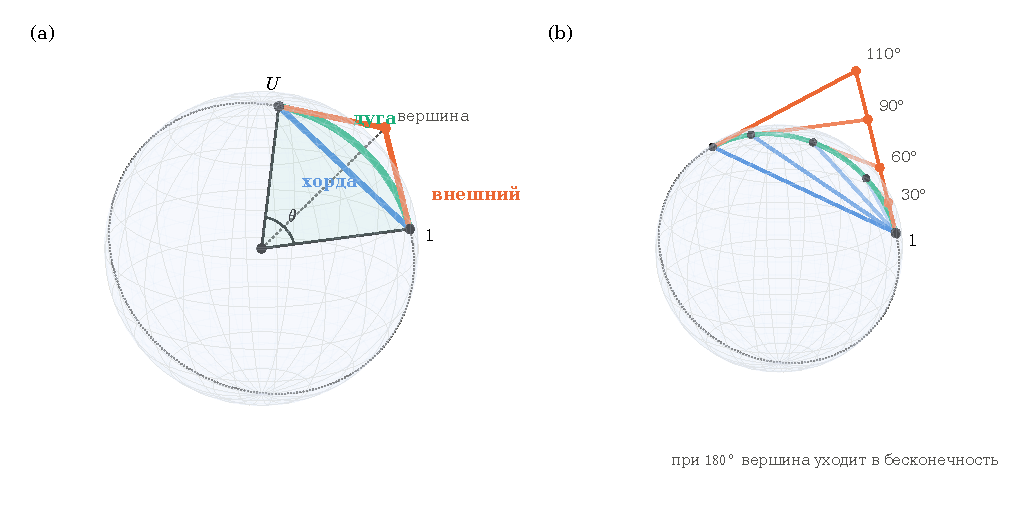
\includegraphics[width=\linewidth]{figures/fig_sphere_3d.pdf}
\caption{Три пути в трёх измерениях. \textbf{(a)} Поворот на $\theta=70^\circ$ в плоскости,
проходящей через центр единичной сферы: дуга (зелёная) идёт по поверхности, хорда (синяя)
проходит сквозь внутренность, а внешний путь (оранжевый) уходит по касательной в точке $1$,
поворачивает в вершине на биссектрисе на расстоянии $\sec(\theta/2)$ и возвращается по касательной
в точке $U$. \textbf{(b)} Повороты на $30^\circ$, $60^\circ$, $90^\circ$ и $110^\circ$ из одного и того же
начального положения. Хорда и дуга остаются ограниченными; вершина уходит наружу вдоль биссектрисы и
достигает бесконечности при полуобороте~--- это тот барьер, который снова встретится в разделах~\ref{sec:energy}
и~\ref{sec:su2}. Ортографическая проекция; построено скриптом \texttt{make\_figures.py}.}
\label{fig:sphere}
\end{figure}

\paragraph{Что здесь классическое и что добавляет эта работа.} Неравенство $C<A<T$~---
это архимедово зажатие окружности между вписанными и описанными многоугольниками
\cite{archimedes}. Взвешенная комбинация из раздела~\ref{sec:lengths}~--- это
оценка Снеллиуса~--- Гюйгенса \cite{snellius,huygens}. Энергия хорды есть действие Вильсона на решётке
\cite{wilson}, энергия дуги~--- действие Мантона \cite{manton}, отображение Кэли относится к
1846 году \cite{cayley}, а метод Кранка~--- Николсон~--- к 1947 году \cite{cn}. Ни одно из этих
отождествлений не ново. Эта работа читает три пути как один объект: три
способа измерить один и тот же поворот, которые промахиваются в фиксированных пропорциях, причём каждая пропорция
снова проявляется в энергии, в алгебре и в шагах по времени. Затем проверяется, насколько
это существенно на реальной неабелевой сетке. Часть истории с энергией тоже не нова.
Сокращение члена $\theta^4$ (вклада компактности) в действии Вильсона уже выполнялось для $U(1)$
с помощью присоединённого члена с удвоенным углом \cite{deforcrand}. Для $U(1)$ и $SU(2)$
касательная энергия в виде $T^2/2$ совпадает с сохраняющим топологию действием Люшера при его
граничном значении \cite{luscher,fukaya}. Скалярное неравенство
$\tfrac23(\sin x/x)^2+\tfrac13(\tan x/x)^2>1$, стоящее за предложением~\ref{prop:energy},~--- известное
неравенство типа Уилкера~--- Гюйгенса \cite{wusrivastava,yang}, а хорда, дуга и касательная
встречаются рядом как дискретные кривизны многоугольников \cite{cranewardetzky}. Чего мы не нашли,
так это самой смеси хорды и касательной, предложенной как решёточная энергия, её алгебраической
записи через $U$ и её коэффициентов $\tfrac{7}{720}$ и $\tfrac{1}{1008}$.

\paragraph{Куда это ведёт.} Поворот в этой работе~--- не только палочка на окружности. В
калибровочном поле каждая малая петля несёт такой поворот~--- свою голономию, и при таком прочтении картинка
говорит три вещи. Поворот создаёт энергию: петля, которая не повернулась, ничего не стоит,
и энергия петли~--- это то, насколько она повернулась. Два конца поворота достигают друг друга
через внутренность: решётка измеряет хорду, потому что дуга~--- это путь, по которому может пройти
только само вращение. И наименьшая единица поворота искривлена, потому что она существует:
одна единица, простирающаяся одинаково во всех направлениях, есть сфера, а в четырёх измерениях эта
сфера есть $SU(2)$~--- группа, из которой построено поле Янга~--- Миллса. В сопутствующей работе
\emph{Читать кривую, а не считать точки}~\cite{davis-rtc} вычисления с этими поворотами проводятся
на сетках гомологической сферы Пуанкаре. В разделе~\ref{sec:mesh} измеряется, насколько
три пути различаются там, а раздел~\ref{sec:ym} возвращается к тому, что они подсказывают о
теории Янга~--- Миллса. В разделе~\ref{sec:claims} сказано, как далеко заходит эта работа и где она останавливается.
